\documentclass[UTF8,a4paper,twocolumn,zihao=5,fontset=none]{ctexart}

\usepackage[left=23mm,right=23mm,top=19mm,bottom=20mm,headsep=4mm,footskip=9mm]{geometry}
\setlength{\columnsep}{7.5mm}
\usepackage{fontspec}
\usepackage{unicode-math}
\setCJKmainfont[Path=C:/Windows/Fonts/]{simsun.ttc}
\setmainfont[
  Path=C:/Windows/Fonts/,
  BoldFont=timesbd.ttf,
  ItalicFont=timesi.ttf,
  BoldItalicFont=timesbi.ttf
]{times.ttf}
\setmathfont[Path=D:/MiKTeX/texmfs/texmfs/install/fonts/opentype/public/stix2-otf/]{STIXTwoMath-Regular.otf}
\usepackage{graphicx}
\usepackage{booktabs}
\usepackage{array}
\usepackage{amsmath}
\usepackage{siunitx}
\usepackage{caption}
\usepackage{float}
\usepackage{dblfloatfix}
\usepackage{placeins}
\usepackage{microtype}
\usepackage[hidelinks]{hyperref}
\usepackage[numbers,sort&compress]{natbib}

\graphicspath{{../../figures/paper/}}
\linespread{1.20}
\setlength{\parindent}{2em}
\setlength{\parskip}{0pt}
\setlength{\textfloatsep}{7pt plus 2pt minus 2pt}
\setlength{\floatsep}{6pt plus 2pt minus 2pt}
\setlength{\intextsep}{6pt plus 2pt minus 2pt}
\renewcommand{\topfraction}{0.92}
\renewcommand{\bottomfraction}{0.85}
\renewcommand{\textfraction}{0.06}
\renewcommand{\floatpagefraction}{0.82}
\renewcommand{\dbltopfraction}{0.92}
\renewcommand{\dblfloatpagefraction}{0.82}
\captionsetup{font=small,labelfont=bf,labelsep=quad,skip=3pt}
\renewcommand{\figurename}{图}
\renewcommand{\tablename}{表}
\ctexset{
  section={format=\bfseries\zihao{4},beforeskip=0.8ex,afterskip=0.45ex},
  subsection={format=\bfseries\zihao{-4},beforeskip=0.6ex,afterskip=0.3ex}
}

\newcommand{\engcaption}[1]{\par\vspace{-0.2em}{\centering\zihao{-5}\rmfamily #1\par}}
\newcommand{\figurenote}[2]{\par\vspace{0.15em}{\zihao{6}#1\par}}
\newcommand{\tablenote}[2]{\par\vspace{0.2em}{\zihao{6}注：#1\par\rmfamily Note: #2\par}}
\newcommand{\Rtwo}{\ensuremath{R^{2}}}

\title{\bfseries\zihao{2}基于多模型融合与可解释学习的工业蒸汽量预测方法\\[0.45em]
{\zihao{3}\rmfamily Industrial Steam Prediction Based on Multi-model Fusion and Interpretable Learning}}
% TODO: replace with real author information
\author{\zihao{4}作者1，作者2\\[-0.1em]\zihao{5}（单位名称，城市\ 邮编）}
\date{}

\begin{document}
\twocolumn[
\maketitle
\vspace{-2.0em}
\begin{center}
\begin{minipage}{164mm}
\zihao{5}
\noindent\textbf{摘要：}针对 38 维匿名过程特征条件下的工业蒸汽量回归预测问题，构建包含线性模型、树模型、特征处理、参数搜索、模型融合及解释诊断的统一实验流程。主实验采用 5 折 TimeSeriesSplit，并以 KFold 作为敏感性分析。结果表明，Best Ridge 的 MSE、RMSE、MAE 和 \Rtwo 分别为0.1304、0.3593、0.2639和0.8525；在含 481 个样本的独立融合验证集上，Weighted Blend 对应指标为0.1766、0.420、0.287和0.819。其 MSE 相比 Best Ridge 仅降低约0.19\%，属于边际数值改善。SHAP 分析仅针对 Best XGBoost 分支，V0、V1 位于全局贡献幅度前列。残差诊断显示多数预测接近观测值，但尾部仍有较大偏差。研究说明 Ridge 在当前数据和验证设置下具有较强竞争力，融合收益有限，结论尚不支持统计显著性推断。

\vspace{0.35em}\noindent\textbf{关键词：}工业蒸汽量预测；机器学习；Ridge回归；XGBoost；模型融合；SHAP；时间序列交叉验证

\vspace{0.55em}\noindent\textbf{Abstract:} A unified workflow integrating linear and tree-based regressors, feature processing, hyperparameter search, model fusion, and diagnostic interpretation is developed for industrial steam prediction from 38 anonymous features. Five-fold TimeSeriesSplit is used for the main evaluation, with KFold serving only as a sensitivity analysis. Best Ridge obtains MSE, RMSE, MAE, and $R^2$ values of 0.1304, 0.3593, 0.2639, and 0.8525. On an independent fusion validation set of 481 samples, Weighted Blend obtains 0.1766, 0.420, 0.287, and 0.819, respectively. Its MSE is only about 0.19\% lower than that of Best Ridge, indicating a marginal numerical gain. SHAP analysis is restricted to the Best XGBoost branch. Residual diagnostics reveal that tail errors remain.

\vspace{0.25em}\noindent\textbf{Key words:} industrial steam prediction; machine learning; Ridge regression; XGBoost; model fusion; SHAP; time-series cross-validation
\end{minipage}
\end{center}
\vspace{0.8em}
]

\section{引言}
工业过程中的关键质量、产量或能耗变量有时难以在线直接测量，数据驱动软测量可利用较易获得的过程变量建立目标变量的回归映射，为运行评估、参数调整和生产决策提供定量依据。Kadlec等\citep{kadlec2009softsensor}系统总结了过程工业数据驱动软测量的建模特点与应用问题。后续综述指出，工业数据往往同时具有高维、非线性、动态变化、变量相关及标签稀缺等特征，模型还需适应局部工况和数据分布变化\citep{yeo2023jit,sheng2024review}。人工智能驱动软测量在过程监测和可持续运行中具有应用价值，但其可靠性仍依赖数据质量、验证设计和部署条件\citep{perera2023ai_softsensor}。

针对不同数据结构，已有研究采用树模型、深度网络、混合模型和特征处理策略开展工业过程预测。例如，Seq2Seq 与 LightGBM 的组合用于动态软测量\citep{li2020seq2seq_lightgbm}，Random Forest 被用于工业精馏装置的在线软测量实现\citep{botha2021industrial_softsensor}，基于 Random Forest 的特征选择也被用于发酵过程预测\citep{hua2023rf_feature_selection}。在复杂工业过程中，两层集成框架、即时集成学习及带注意力的多输出 Random Forest 分别用于利用模型互补性或多变量结构\citep{wang2019two_layer_ensemble,pan2019ensemble_jit,wan2024wide_rf}。《浙江大学学报（工学版）》中的 XGBoost 风电功率预测和跨维度特征融合寿命预测研究也表明，树模型与特征融合可服务于不同工程预测任务\citep{wang2023zju_wind_xgboost,zhang2025zju_feature_fusion}。这些工作提供了方法参照，但任务、变量语义和评估协议并不相同，复杂模型因而不能被预设为在所有工业数据上优于线性正则模型。

单模型具有不同的偏差与方差特征，ensemble 与 Stacking 可通过组合预测利用有限互补性；其收益仍取决于基模型质量、权重估计及验证集设计。工业软测量中的两层集成和即时集成研究展示了这种建模思路\citep{wang2019two_layer_ensemble,pan2019ensemble_jit}，Stacking 的基本框架由 Wolpert 提出\citep{wolpert1992stacking}，同刊近期研究则将多模型 Stacking 用于基坑时序预测\citep{hu2025zju_stacking}。除平均误差外，工业预测还需说明模型依据及尾部风险。SHAP 建立了统一的加性特征归因框架\citep{lundberg2017shap}，并已用于树集成和 Informer 工业软测量的解释\citep{cao2023interpretable_softsensor,cao2024informer_shap}；同刊工程研究也给出了 XGBoost--SHAP 在承载力预测和非线性影响分析中的应用\citep{chen2023zju_xgboost_shap,lu2025zju_xgboost_shap}。上述研究说明 SHAP 可用于解释特定模型输出，但本文仅将其用于 Best XGBoost 分支，不解释 Weighted Blend 或完整融合系统。

对于本文的 38 维匿名特征工业蒸汽量任务，仍需在统一评估口径下回答：线性正则模型与多种树模型何者更稳健，KBest 和 PCA 是否带来收益，Ridge 正则化强度如何影响误差，融合模型能够获得多大实际改善，以及如何在不扩大解释边界的前提下分析特征贡献与残差。本文不提出新的学习算法，而是构建口径一致、可复核的实验流程：1）在统一 5 折 TimeSeriesSplit 协议下比较 Ridge、XGBoost、GBDT、LightGBM 和 Random Forest；2）分析 KBest、PCA 及 Ridge 正则化参数的性能敏感性；3）在独立融合验证集上比较 Weighted Blend 与 Stacking，并量化融合收益边界；4）结合 SHAP 和残差诊断，分别分析 Best XGBoost 的全局特征贡献与 Weighted Blend 的误差结构。同刊相关研究仅作为工程方法参照\citep{chen2023zju_xgboost_shap,hu2025zju_stacking,zhang2025zju_feature_fusion,lu2025zju_xgboost_shap}，本文不在不同任务和数据集之间作性能优劣比较。

\section{数据与问题定义}
\subsection{数据集与变量}
训练集包含2 888行、39列，其中输入变量为匿名特征 V0--V37，响应变量为 target；测试集包含1 925行、38列且不提供 target。由于缺少变量物理语义，本文不将 V0--V37解释为温度、压力、流量或其他具体工艺量，也不报告无标签测试集上的预测性能。

如图\ref{fig:target}所示，target 的均值和中位数分别为0.126和0.313，主体样本集中于中间区域，同时两侧均有尾部。这一分布提供了理解后续 MSE、MAE 及尾部残差的尺度背景，但不承担模型优劣判断。

\begin{figure}[t]
  \centering
  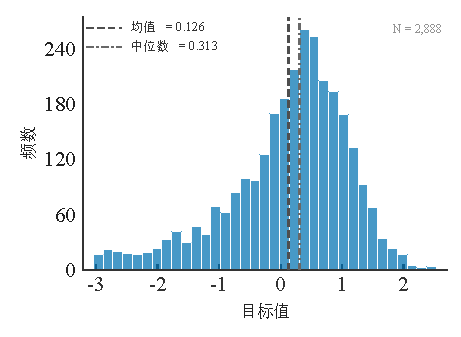
\includegraphics[width=\columnwidth]{fig1_target_distribution_zh.pdf}
  \caption{工业蒸汽量目标变量的分布}
  \label{fig:target}
  \engcaption{Fig.1 Distribution of industrial steam target variable}
\end{figure}

\subsection{数据质量检查}
当前冻结的数据质量检查结果表明，训练数据中无缺失值、无重复行且无无穷值。该检查仅说明表层完整性，不等同于确认采样时间、工况切换或传感器语义。特别地，现有元数据尚不足以严格确认数据行顺序的时间含义，故验证策略的解释需保持谨慎。

\subsection{预测任务定义}
令 $\boldsymbol{x}_i\in\mathbb{R}^{38}$ 表示第 $i$ 个样本的匿名特征向量，$y_i$ 表示工业蒸汽量目标值，回归模型 $f(\cdot)$ 输出 $\hat y_i=f(\boldsymbol{x}_i)$。目标是在明确的验证协议下减小预测误差，同时通过模型比较、敏感性分析和诊断图识别性能边界。

\section{预测方法}
\subsection{Ridge 回归}
数据首先经标准化处理，再训练 Ridge 模型。Ridge通过二次惩罚项收缩相关变量的回归系数\citep{hoerl1970ridge}，其优化目标为
\begin{equation}
 \min_{\boldsymbol{\beta}}\ \lVert\boldsymbol{y}-\boldsymbol{X}\boldsymbol{\beta}\rVert_2^2+\alpha\lVert\boldsymbol{\beta}\rVert_2^2,
\end{equation}
其中 $\alpha$ 控制系数收缩强度。本文在给定搜索范围内比较多个 $\alpha$，最终观测到 $\alpha = 5$ 时平均交叉验证 MSE 最低，但其相对邻近参数仅为浅幅数值最优。

\subsection{树模型}
树模型包括 XGBoost、GBDT、LightGBM 和 Random Forest，其方法基础分别参见文献\citep{chen2016xgboost,friedman2001gbdt,ke2017lightgbm,breiman2001randomforest}。Best XGBoost 采用300棵树、学习率0.05、最大深度2、子采样率0.8和列采样率1.0，随机种子为42。本文将这些模型置于相同主验证口径下比较，不因模型复杂度预设其优越性。

\subsection{特征处理方法}
比较三种输入策略：使用全部 38 个特征、通过单变量筛选保留 20 个特征（KBest20）以及保留 95\% 累计解释方差的主成分（PCA95）。特征选择的一般目标与方法分类参见文献\citep{guyon2003feature_selection}，PCA 的理论与近期综述参见文献\citep{jolliffe2016pca}。所有策略均与 Ridge 组合，目的在于检验降维或筛选在当前数据和验证设置下是否带来数值收益，而非推断特征选择方法普遍有效或无效。

\subsection{超参数优化}
Ridge 的 $\alpha$ 候选值为0.01、0.1、0.5、1、2、5、10、20、50和100。XGBoost 通过既定搜索过程得到上述 Best XGBoost 配置。调参前后性能在相同 5 折 TimeSeriesSplit 口径下汇总，以避免将不同协议下的结果直接混合。

\subsection{加权融合与 Stacking}
Weighted Blend 对 Best Ridge 和 Best XGBoost 的预测作线性组合：
\begin{equation}
 \hat y_{\mathrm{blend}}=w_{\mathrm{Ridge}}\hat y_{\mathrm{Ridge}}+w_{\mathrm{XGB}}\hat y_{\mathrm{XGB}}.
\end{equation}
权重搜索最终选取 $w_{\mathrm{Ridge}}=0.7$、$w_{\mathrm{XGB}}=0.3$。最终性能仅引用独立融合验证集结果，不使用同一候选池上更乐观的融合搜索数值。Stacking遵循堆叠泛化的基本思想\citep{wolpert1992stacking}，作为另一融合基线与上述模型在相同独立验证集上比较。

\subsection{SHAP解释方法}
SHAP 基于可加性特征归因框架\citep{lundberg2017shap}。本文仅使用平均绝对 SHAP 值描述 Best XGBoost 分支的全局贡献幅度。该量不提供影响方向，不能建立因果关系，也不表示统计显著性；因此 SHAP 结果不用于直接解释 Weighted Blend 或完整融合系统。

\section{实验设计}
\subsection{评价指标}
对 $N$ 个样本，采用
\begin{align}
 \mathrm{MSE}&=\frac{1}{N}\sum_{i=1}^{N}(y_i-\hat y_i)^2,\\
 \mathrm{RMSE}&=\sqrt{\mathrm{MSE}},\\
 \mathrm{MAE}&=\frac{1}{N}\sum_{i=1}^{N}|y_i-\hat y_i|,\\
 R^2&=1-\frac{\sum_i(y_i-\hat y_i)^2}{\sum_i(y_i-\bar y)^2}.
\end{align}
MSE、RMSE 和 MAE 越小越好，\Rtwo 越大表示解释的目标波动比例越高。本文未进行显著性检验，折间标准差也不被解释为置信区间。

\subsection{验证策略}
时间序列预测的交叉验证需要考虑观测顺序与相关结构，不同划分方式可能改变性能估计\citep{bergmeir2012cv}；对自回归预测交叉验证有效性的讨论也表明，结论依赖具体数据生成与建模条件\citep{bergmeir2018cv}。为降低潜在顺序相关性引起的信息泄漏风险，本文主实验采用 5 折 TimeSeriesSplit，同时使用 KFold 进行敏感性分析。Best Ridge 在 TimeSeriesSplit 下的 MSE 为0.1304，在 KFold 下为0.1129。由于数据行顺序的严格时间语义尚未由元数据充分确认，二者差异仅说明结果对划分方式敏感，不能证明 TimeSeriesSplit 是唯一正确策略，也不表示 KFold 本身错误。

\subsection{模型与参数设置}
各模型使用统一评价指标。Ridge 在标准化后拟合，Best Ridge 的 $\alpha = 5$；Best XGBoost 参数如 3.2 节所述。图\ref{fig:model}和表\ref{tab:model}报告主验证结果，图中误差棒为 5 折间的一个标准差，而非置信区间。

\subsection{融合验证协议}
融合比较使用独立的481样本验证集，并在同一集合上评价 Weighted Blend、Best Ridge、Stacking 和 Best XGBoost。该口径与表\ref{tab:model}的5折均值不同，故表\ref{tab:fusion}不能与表\ref{tab:model}进行直接横向数值比较。

\section{结果与分析}
\subsection{目标变量分布}
图\ref{fig:target}使用全部2 888个训练样本，并按 Freedman-Diaconis 规则确定直方图分箱；虚线和点划线分别标示均值0.126和中位数0.313。目标变量具有明显主体区间和双侧尾部，尾部样本全部保留，因此后续误差统计包含这些较难预测的观测。均值低于中位数只是分布位置的描述，本文未据此拟合参数分布或作显著性判断。

\subsection{基础模型性能比较}
由图\ref{fig:model}可知，Best Ridge 的平均 MSE 最低，为0.1304；普通 Ridge 与其数值非常接近。Best XGBoost 调参后有所改善，但仍未超过 Ridge 系列。误差棒表示 5 折 TimeSeriesSplit 结果的 $\pm 1$ 个标准差，而非置信区间；其重叠情况不用于显著性判断。

\begin{figure}[t]
  \centering
  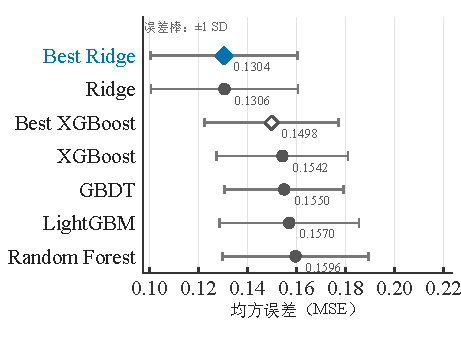
\includegraphics[width=\columnwidth]{fig2_model_performance_zh.pdf}
  \caption{不同回归模型在 5 折 TimeSeriesSplit 验证下的预测性能}
  \label{fig:model}
  \engcaption{Fig.2 Prediction performance of regression models under five-fold TimeSeriesSplit validation}
  \figurenote{误差棒为 5 折 TimeSeriesSplit 结果的 $\pm 1$ SD。}{}
\end{figure}

\begin{table}[t]
\centering
\caption{不同回归模型的 5 折 TimeSeriesSplit 验证性能}
\label{tab:model}
\engcaption{Table 1 Prediction performance of regression models under five-fold TimeSeriesSplit validation}
\zihao{6}\setlength{\tabcolsep}{3.1pt}
\begin{tabular}{lrrrr}
\toprule
模型 & MSE & RMSE & MAE & \Rtwo \\
\midrule
Best Ridge & \textbf{0.1304} & \textbf{0.3593} & \textbf{0.2639} & \textbf{0.8525} \\
Ridge & 0.1306 & 0.3595 & 0.2643 & 0.8523 \\
Best XGBoost & 0.1498 & 0.3858 & 0.2888 & 0.8261 \\
XGBoost & 0.1542 & 0.3915 & 0.2952 & 0.8203 \\
GBDT & 0.1550 & 0.3927 & 0.2964 & 0.8207 \\
LightGBM & 0.1570 & 0.3950 & 0.2990 & 0.8186 \\
Random Forest & 0.1596 & 0.3981 & 0.2997 & 0.8164 \\
\bottomrule
\end{tabular}
\tablenote{各指标均为 5 折 TimeSeriesSplit 验证结果的平均值。}{Metrics are means over five TimeSeriesSplit folds.}
\end{table}

表\ref{tab:model}给出完整指标。Best Ridge 的 MSE、RMSE、MAE 和 \Rtwo 分别为0.1304、0.3593、0.2639和0.8525。该结果表明线性正则模型是当前数据上的强基线，但不能外推为对所有工业数据均优于树模型。

\subsection{特征处理与 Ridge 参数敏感性}
图\ref{fig:feature}（a）和表\ref{tab:feature}表明，在当前数据集及验证设置下，使用全部38个特征的 Ridge 的 MSE 最低；KBest20 和 PCA95 均未带来改善。该结论仅限定于当前实验，不表示特征筛选或降维普遍无效。

\begin{figure*}[t]
  \centering
  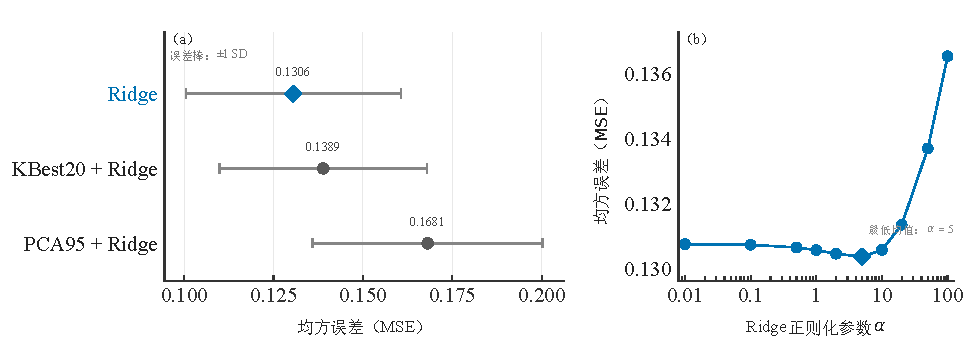
\includegraphics[width=\textwidth]{fig3_feature_ridge_sensitivity_zh.pdf}
  \caption{特征处理方法和 Ridge 正则化参数对预测误差的影响}
  \label{fig:feature}
  \engcaption{Fig.3 Effects of feature processing and Ridge regularization parameter on prediction error}
  \figurenote{（a）误差棒为 5 折 TimeSeriesSplit 结果的 $\pm 1$ SD；（b）仅显示平均交叉验证 MSE。}{}
\end{figure*}

\begin{table}[t]
\centering
\caption{不同特征处理方法下 Ridge 模型的预测性能}
\label{tab:feature}
\engcaption{Table 2 Prediction performance of Ridge under different feature-processing strategies}
\zihao{6}\setlength{\tabcolsep}{3.3pt}
\begin{tabular}{lrrrr}
\toprule
特征处理方法 & MSE & RMSE & MAE & \Rtwo \\
\midrule
Ridge & \textbf{0.1306} & \textbf{0.3595} & \textbf{0.2643} & \textbf{0.8523} \\
KBest20 + Ridge & 0.1389 & 0.3711 & 0.2736 & 0.8424 \\
PCA95 + Ridge & 0.1681 & 0.4085 & 0.3116 & 0.8074 \\
\bottomrule
\end{tabular}
\tablenote{各指标均为当前 5 折 TimeSeriesSplit 验证结果的平均值。}{Metrics are means under the current five-fold TimeSeriesSplit setting.}
\end{table}

图\ref{fig:feature}（b）显示，$\alpha$ 在0.01至10的较宽范围内平均 MSE 变化较小；$\alpha = 5$ 对应最低观测均值0.1304，但与 $\alpha = 1$ 等邻近设置的差距很小。当 $\alpha$ 增至20、50和100时，MSE 逐步升高。子图仅呈现均值趋势，折间标准差未绘入，因此不作显著性判断。

表\ref{tab:tuning}进一步比较调参前后结果。Ridge 调参收益很小；XGBoost 的 MSE 从0.1542降至0.1498，改善幅度相对更清楚，但仍高于 Ridge 系列。

\begin{table}[t]
\centering
\caption{Ridge 与 XGBoost 调参前后的预测性能}
\label{tab:tuning}
\engcaption{Table 3 Prediction performance before and after tuning Ridge and XGBoost}
\zihao{6}\setlength{\tabcolsep}{3.7pt}
\begin{tabular}{lrrrr}
\toprule
模型 & MSE & RMSE & MAE & \Rtwo \\
\midrule
Ridge & 0.1306 & 0.3595 & 0.2643 & 0.8523 \\
Best Ridge & \textbf{0.1304} & \textbf{0.3593} & \textbf{0.2639} & \textbf{0.8525} \\
XGBoost & 0.1542 & 0.3915 & 0.2952 & 0.8203 \\
Best XGBoost & 0.1498 & 0.3858 & 0.2888 & 0.8261 \\
\bottomrule
\end{tabular}
\tablenote{调参前后结果均采用相同的 5 折 TimeSeriesSplit 评估口径。}{All entries use the same five-fold TimeSeriesSplit protocol.}
\end{table}

\subsection{融合模型性能}
图\ref{fig:fusion}和表\ref{tab:fusion}给出独立融合验证集结果。Weighted Blend 的 MSE 为0.1766，略低于 Best Ridge 的0.1769；相对降低约0.19\%，属于边际数值改善。Stacking 略差于 Best Ridge，Best XGBoost 在该集合上的误差最高。

\begin{figure}[t]
  \centering
  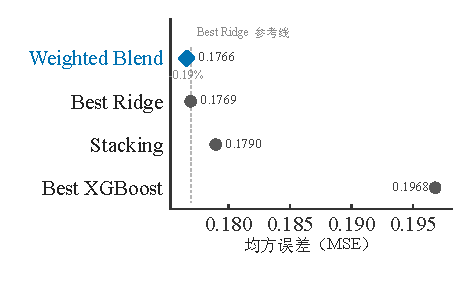
\includegraphics[width=\columnwidth]{fig4_fusion_comparison_zh.pdf}
  \caption{独立融合验证集上不同模型的均方误差比较}
  \label{fig:fusion}
  \engcaption{Fig.4 Comparison of model mean squared errors on independent fusion validation set}
\end{figure}

\begin{table}[t]
\centering
\caption{独立融合验证集上的融合模型性能}
\label{tab:fusion}
\engcaption{Table 4 Fusion model performance on the independent fusion validation set}
\zihao{6}\setlength{\tabcolsep}{3.5pt}
\begin{tabular}{lrrrr}
\toprule
模型 & MSE & RMSE & MAE & \Rtwo \\
\midrule
Weighted Blend & \textbf{0.1766} & \textbf{0.4202} & \textbf{0.2870} & \textbf{0.8190} \\
Best Ridge & 0.1769 & 0.4206 & 0.2882 & 0.8186 \\
Stacking & 0.1790 & 0.4230 & 0.2905 & 0.8166 \\
Best XGBoost & 0.1968 & 0.4436 & 0.3032 & 0.7983 \\
\bottomrule
\end{tabular}
\tablenote{该表采用独立融合验证集，与表\ref{tab:model}的5折交叉验证评估口径不同。}{This independent-validation protocol differs from that of Table~\ref{tab:model}.}
\end{table}

由于没有独立重复实验或置信区间，当前结果不足以认定 Weighted Blend 与 Best Ridge 之间存在统计差异。融合结果的意义更接近于验证两类模型输出具有有限互补性，而非构成实质性性能突破。

\subsection{SHAP特征重要性}
图\ref{fig:shap}显示 Best XGBoost 分支的前 15 个全局 SHAP 特征。V0 的平均绝对 SHAP 值最高（0.329），V1 次之（0.179），随后贡献幅度快速下降，说明该分支的预测贡献呈头部集中。

\begin{figure}[!htbp]
  \centering
  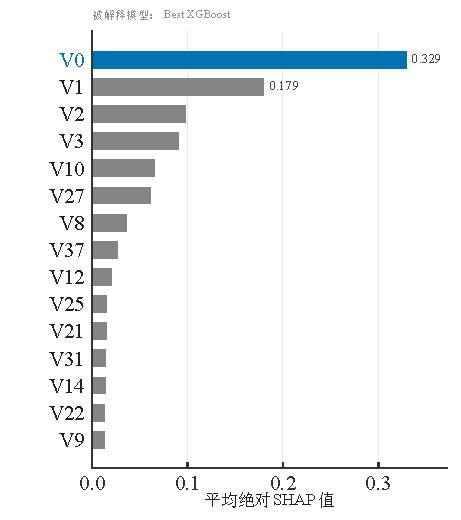
\includegraphics[width=\columnwidth]{fig5_shap_importance_zh.pdf}
  \caption{Best XGBoost 模型的全局 SHAP 特征重要性}
  \label{fig:shap}
  \engcaption{Fig.5 Global SHAP feature importance of Best XGBoost model}
\end{figure}

由于输入变量匿名，V0 不能被称为“最重要工业过程变量”。此外，平均绝对 SHAP 值不包含正负方向，亦不能将头部集中解释为因果机制。该分析仅补充 Best XGBoost 的全局归因结构。

\subsection{预测误差与残差诊断}
图\ref{fig:diag}对应 Weighted Blend 在独立融合验证集上的全部 481 个样本，其 MSE、RMSE、MAE 和 \Rtwo 分别为0.1766、0.420、0.287和0.819。图\ref{fig:diag}（a）中大多数点接近 $y=x$ 参考线，但仍有少量较大偏差；图\ref{fig:diag}（b）显示残差分布于零值两侧并具有较长正残差尾部，图\ref{fig:diag}（c）进一步呈现集中区域与尾部。所有样本均被保留，融合没有消除所有极端预测误差。

\begin{figure*}[!t]
  \centering
  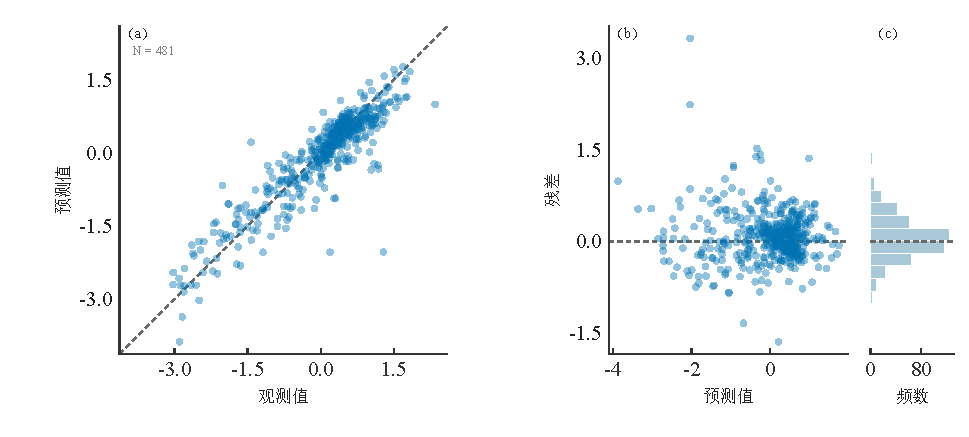
\includegraphics[width=\textwidth]{fig6_prediction_diagnostics_zh.pdf}
  \caption{Weighted Blend 模型在独立融合验证集上的预测与残差诊断}
  \label{fig:diag}
  \engcaption{Fig.6 Prediction and residual diagnostics of Weighted Blend on independent fusion validation set}
\end{figure*}

\subsection{讨论}
结果首先说明，Ridge 在当前匿名特征数据上具有较强基线竞争力，复杂树模型并未自动取得更低误差。其次，KBest20 和 PCA95 在当前设置下没有改善 Ridge，而 $\alpha = 5$ 仅为浅幅数值最优。再次，Weighted Blend 在独立融合验证集上取得最低 MSE，但相对 Best Ridge 的改善仅约0.19\%，当前没有独立重复实验支持统计显著性结论。

本研究仍有多项限制。其一，特征为匿名变量，物理机理解释受到限制；其二，数据行顺序的严格时间语义尚未完全确认，TimeSeriesSplit 旨在降低潜在泄漏风险，但并非被证明为唯一合理策略；其三，SHAP 仅解释 Best XGBoost 分支，不能推广为融合模型的整体解释；其四，残差尾部仍存在较大误差；其五，无标签测试集不能提供真实泛化指标。后续需在明确时间戳、工况含义和外部标签的数据上开展重复实验，并检验模型在其他工业工况或数据集上的泛化能力。

\section{结论}
本文构建了工业蒸汽量预测的统一实验流程。Best Ridge 在主验证中取得最低平均 MSE，$\alpha = 5$ 是当前搜索范围内的浅幅数值最优；特征筛选与 PCA 未改善当前 Ridge 性能。Weighted Blend 在独立融合验证集上取得最低 MSE，但相对 Best Ridge 仅改善约0.19\%。Best XGBoost 的 SHAP 贡献集中于少数匿名特征，预测诊断则显示尾部误差仍未消除。因而，当前证据支持将 Ridge 视为强基线，并将融合收益界定为边际数值改善，而不作显著性或普适性推断。

% TODO: replace with actual funding information when available.
% TODO: replace author affiliations and corresponding-author details.

\FloatBarrier
{\zihao{6}
\bibliographystyle{unsrtnat}
\bibliography{references}
}

\end{document}
